%% The following is a directive for TeXShop to indicate the main file
%%!TEX root = diss.tex

\chapter{Identification of Germline Variants in FFPE Tumours}
\label{ch:IdentificationofGermlineVariantsinFFPETumours}

Tumour-only sequencing is commonly adopted by clinical laboratories for detection of targetable somatic mutations. Unlike the research setting, matched normal samples such as blood, saliva, or adjacent normal tissues are not routinely processed by clinical laboratories to minimize cost and turnaround time. The tumour genome also contains germline information that may have clinical implications for patients and their families. For instance, germline variants in cancer-predisposing genes could facilitate implementation of cancer preventative measures and routine surveillance. Moreover, germline alterations in PGx genes could predict response to drug treatment such as chemotherapeutic agents, thereby preventing adverse drug reactions.

Because the tumour genome consists of both germline and somatic changes, it is important to establish approaches to distinguish between germline and somatic alterations in tumour-only sequencing assays. Subsequently, potential germline variants can be referred to downstream confirmatory testing, which involves genetic counseling and acquisition of germline samples for sequencing and analysis.

The TOP study is comprised of 213 patients with tumour and matched blood specimens. To determine whether tumour DNA can be

- Our study has matched specimens, which allows us to identify true germline alterations from the tumour genome through matched analyses.
- This allow us to calculate true positive rates of our approaches to distinguish between germline and somatic alterations in the tumour genome.
-  How good are our methods?

Using blood We first determined the frequency of germline variants in patients from the TOP cohort and the concordance of germline variants between FFPE tumours and blood, which is

compared different bioinformatics approaches in distinguishing between

%%%%%%%%%%%%%%%%%%%%%%%%%%%%%%%%%%%%%%%%%%%%%%%%%%%%%%%%%%%%%%%%%%%%%
\section{Frequency and characteristics of germline variants in patients from TOP cohort}
\label{sec:FrequencyandcharacteristicsofgermlinevariantsinpatientsfromTOPcohort}
%%%%%%%%%%%%%%%%%%%%%%%%%%%%%%%%%%%%%%%%%%%%%%%%%%%%%%%%%%%%%%%%%%%%%

We analyzed the germline variants detected in blood specimens of 213 patients and identified a total of  germline variants.



%%%%%%%%%%%%%%%%%%%%%%%%%%%%%%%%%%%%%%%%%%%%%%%%%%%%%%%%%%%%%%%%%%%%%%
%%%%%%%%%%%%%%%%%%%%%%%%%%%%%%%%%%%%%%%%%%%%%%%%%%%%%%%%%%%%%%%%%%%%%%

\begin{landscape}

\begin{longtable}{p{0.07\linewidth}|p{0.09\linewidth}p{0.11\linewidth}p{0.1\linewidth}p{0.05\linewidth}p{0.065\linewidth}p{0.11\linewidth}p{0.25\linewidth}p{0.05\linewidth}}
		\caption{Description of germline variants in cancer genes detected in blood specimens of TOP patients.}
    \label{tbl:germline_cancer_genes}
		\\
    \hline
    Gene & Chr:Pos & ID\textsuperscript{$\star$} & HGVS\textsuperscript{*} & AF\textsuperscript{**} & Variant Effect\textsuperscript{$\dagger$} & Clinical Significance\textsuperscript{$\dagger\dagger$} & Functional/Clinical Impacts & Ref.
		\\
    \hline
		ALK & 2:29443662 & NA & p.Val1185Val c.3555G$>$A & 0.00082 & Syn. & NA & NA & NA
		\\
		\\
		\hline
		EGFR & 7:55242453 & NA & p.Pro741Pro c.2223C$>$T & 0.0074 & Syn. & NA & NA & NA
		\\
		\\
		& 7:55242500 & COSM133588 & p.Lys757Arg c.2270A$>$G & 0.00082 & Missense & Uncertain \mbox{significance} & Homozygous mutation was identified in a patient with intrahepatic cholangiocarcinoma, leading to activation of downstream EGFR pathways as demonstrated by MAPK and Akt phosphorylations. & \cite{Leone2006}
		\\
		\\
		& 7:55249063 & rs1050171; COSM1451600\textsuperscript{$\ddagger$} & p.Gln787Gln c.2361G$>$A & 52 & Syn. & Benign/Likely benign & Conflicting evidence on predictive and prognostic values in lung cancer patients. Poorer response to anti-EGFR therapy in colorectal cancer patients compared to patients with the GG genotype. & \cite{Zhang2006a, Leichsenring2017, Wang2013, Bonin2016}
		\\
		\\
		& 7:5524915 & rs56183713; COSM13400 & p.Val819Val c.2457G$>$A & 0.035 & Syn. & Likely benign & One study reported that this variant in combination with rs1050171 was correlated with TNM stage of squamous cell lung carcinoma. & \cite{Wang2013}
		\\
		\\
		& 7:55259450 & rs2229066; COSM85893; rs17290559 & p.Arg836Arg c.2508C$>$T & 1.7 & Syn. & Benign/Likely benign & NA & NA
		\\
		\\
    \hline
		KIT & 4:55592059 & rs151016327; COSM3760661 & p.Thr461Thr c.1383A$>$G & 0.28 & Syn. & Benign & NA & NA
		\\
		\\
		& 4:55599268 & rs55789615; COSM1307 & p.Ile798Ile c.2394C$>$T & 2.1 & Syn. & Benign/Likely benign & NA & NA
		\\
		\\
		& 4:55602765 & rs3733542; COSM1325 & p.Leu862Leu c.2586G$>$C & 12 & Syn. & Benign/Likely benign & NA & NA
		\\
		\\
		\hline
		MAPK1 & 22:22162126 & rs386488966; rs3729910 & p.Tyr43Tyr c.129T$>$C & 4.5 & Syn. & NA & NA & NA
		\\
		\\
		& 22:22221623 & rs201495639 & p.Tyr36Tyr c.108C$>$T & 0.052 & Syn. & NA & NA & NA
		\\
		\\
		\hline
		MTOR & 1:11169420 & rs41274506 & p.Asp2485Asp c.7455C$>$T & 0.33 & Syn. & NA & NA & NA
		\\
		\\
		& 1:11172909 & NA & p.Glu2456Lys c.7366G$>$A & 0.00082 & Missense & NA & NA & NA
		\\
		\\
		& 1:11174452 & NA & p.Arg2408Gln c.7223G$>$A & NA & Missense & NA & NA & NA
		\\
		\\
		& 1:11181327 & rs11121691 & p.Leu2303Leu c.6909G$>$A & 22 & Syn. & NA & Likely has an effect on exonic splicing enhancer or exonic splicing silencer binding site activity. & \cite{Zining2016}
		\\
		\\
		& 1:11184593 & rs56051835 & p.Leu2208Leu c.6624T$>$C & 0.49 & Syn. & Benign & NA & NA
		\\
		\\
		& 1:11188172 & rs370318222 & p.Tyr1974Tyr c.5922C$>$T & 0.00082 & Syn. & NA & NA & NA
		\\
		\\
		& 1:11190646 & rs2275527 & p.Ser1851Ser c.5553C$>$T & 22 & Syn. & Benign & NA & NA
		\\
		\\
		& 1:11190730 & rs17848553 & p.Ala1823Ala c.5469C$>$T & 2.4 & Syn. & Benign & NA & NA
		\\
		\\
		& 1:11194521 & COSM180791 & c.5133C$>$T & 0.029 & Splice region & NA & NA & NA
		\\
		\\
		& 1:11205058 & rs386514433; rs1057079\textsuperscript{$\ddagger$} & p.Ala1577Ala c.4731G$>$A & 68 & Syn. & NA & One study reported improved clinical response and progression-free survival in advanced esophageal squamous cell carcinoma patients with the AG genotype compared to the AA genotype who were treated with paclitaxel plus cisplatin chemotherapy. & \cite{Liu2016}
		\\
		\\
		& 1:11269506 & NA & p.Leu1222Phe c.3664C$>$T & 0.00082 & Missense & NA & NA & NA
		\\
		\\
		& 1:11272468 & rs17036536 & p.Arg1154Arg c.3462G$>$C & 1.8 & Syn. & Benign & NA & NA
		\\
		\\
		& 1:11288758 & rs1064261\textsuperscript{$\ddagger$} & p.Asn999Asn c.2997C$>$T & 74 & Syn. & NA & C allele likely influences exonic splicing enhancer or exonic splicing silencer binding site activity or disrupts a protein domain. Meta-analysis found no association with cancer risk. & \cite{Zining2016}
		\\
		\\
		& 1:11298038 & rs55752564 & p.Ala690Ala c.2070G$>$A & 0.077 & Syn. & NA & NA & NA
		\\
		\\
		& 1:11298640 & rs55881943 & p.Ala607Ala c.1821G$>$A & 0.017 & Syn. & Conflicting \mbox{interpretations} of \mbox{pathogenicity} & NA & NA
		\\
		\\
		& 1:11301714 & rs1135172\textsuperscript{$\ddagger$} & p.Asp479Asp c.1437T$>$C & 72 & Syn. & NA & NA & NA
		\\
		\\
		& 1:11308007 & rs35903812 & p.Ala329Thr c.985G$>$A & 0.27 & Missense & Likely benign & NA & NA
		\\
		\\
		& 1:11316244 & rs12120294 & p.Leu170Leu c.510G$>$C & 0.36 & Syn. & NA & NA & NA
		\\
		\\
		\hline
		PDGFRA & 4:55141055 & rs1873778; COSM1430082\textsuperscript{$\ddagger$} & p.Pro567Pro c.1701A$>$G & 99 & Syn. & Benign & No association with PDGFR$\alpha$ \mbox{expression} in colorectal cancer. & \cite{Estevez-Garcia2012}
		\\
		\\
		& 4:55152040 & rs2228230; COSM22413 & p.Val824Val c.2472C$>$T & 18 & Syn. & Benign & NA & NA
		\\
		\\
		\hline
		STAT1 & 2:191851646 & rs41270237 & p.Thr385Thr c.1155G$>$A & 0.42 & Syn. & Likely benign & NA & NA
		\\
		\\
		& 2:191856001 & rs41509946 & p.Gln330Gln c.990G$>$A & 0.36 & Syn. & Likely benign & NA & NA
		\\
		\\
		& 2:191859906 & rs61756197 & p.Gln275Gln c.825G$>$A & 0.025 & Syn. & NA & NA & NA
		\\
		\\
		& 2:191859935 & rs41473544 & p.Val266Ile c.796G$>$A & 0.20 & Missense & Likely benign & Functional testing indicated that the variant was not a gain-of-function mutation in STAT1 & \cite{Depner2016}
		\\
		\\
		& 2:191872307 & rs45463799 & p.Asn118Asn c.354C$>$T & 0.32 & Syn. & Likely benign & NA & NA
		\\
		\\
		& 2:191874667 & rs386556119; rs2066802 & p.Leu21Leu c.63T$>$C & 8.5 & Syn. & Benign & High frequency among patients with multiple sclerosis and chronic hepatitis C. & \cite{Fortunato2008}
		\\
		\\
		\hline
		STAT3 & 17:40469241 & COSM979464 & c.2100C$>$T & NA & Splice region & NA & NA & NA
		\\
		\\
		& 17:40475056 & rs117691970 & p.Gly618Gly c.1854C$>$T & 0.37 & Syn. & Likely benign & NA & NA
		\\
		\\
		& 17:40486040 & rs200098006 & p.Leu275Leu c.825T$>$G & 0.066 & Syn. & NA & NA & NA
		\\
		\\
		& 17:40486043 & NA & p.Gln274Gln c.822A$>$G & 0.00082 & Syn. & NA & NA & NA
		\\
		\\
		& 17:40498635 & rs146184566; COSM979479 & p.Ser75Ser c.225G$>$A & 0.029 & Syn. & Likely benign & NA & NA
		\\
		\\
		& 17:40498713 & NA & p.Lys49Lys c.147A$>$G & 0.012 & Syn. & NA & NA & NA
		\\
		\\
		& 17:40498722 & NA & p.Ala46Ala c.138G$>$T & NA & Syn. & NA & NA & NA
		\\
		\\
		\hline
		TP53 & 17:7577069 & rs55819519; COSM44017 & p.Arg290His c.869G$>$A & 0.016 & Missense & Conflicting \mbox{interpretations} of \mbox{pathogenicity} & A conservative amino acid substitution that was predicted to be possibly damaging by \textit{in silico} analysis. Reported in patients with Li-Fraumeni syndrome and cancer patients without family histories of Li-Fraumeni syndrome or Li-Fraumeni-like syndrome. & \cite{Chitrala2014, Quesnel1999, Anensen2006, Villani2011, Pennington2013, Arcand2008}
		\\
		\\
		& 17:7577553 & COSM44368 & p.Met243fs c.727delA & NA & Frameshift & NA & Reported in esophageal squamous cell carcinoma of patients from northern Iran. & \cite{Biramijamal2001}
		\\
		\\
		& 17:7578210 & rs1800372; COSM249885 & p.Arg213Arg c.639A$>$G & 1.2 & Syn. & Benign/Likely benign & One study demonstrated that this variant was not a predictive biomarker for initiation and progression of gastroesophageal reflux disease, Barrett's Esophagus, and esophageal cancer in the Brazilian population. & \cite{Pilger2007}
		\\
		\\
		& 17:7578420 & COSM1386804 & p.Thr170Thr c.510G$>$A & 0.012 & Syn. & NA & One study reported that TP53 mutations in exon 5, which include this variant, were associated with the worst prognosis for patients with non-small-cell lung cancer. & \cite{Vega1997}
		\\
		\\
		& 17:7579472 & rs1042522; COSM250061\textsuperscript{$\ddagger$} & p.Pro72Arg c.215C$>$G & 66 & Missense & Drug response & p53 protein with Arg72 was associated with increased apoptosis, while p53 protein with Pro72 demonstrated increased G\textsubscript{1} cell-cycle arrest and activation of p53-dependent DNA repair. Pro/Pro genotype resulted in severe neutropenia in ovarian cancer patients receiving cisplatin-based chemotherapy, and poor survival and treatment response in gastric cancer patients receiving paclitaxel and capecitabine combination chemotherapy, as well as 5-fluorouracil-based adjuvant chemotherapy. Conflicting evidence on risk of predispositon to various cancer types. & \cite{Khrunin2010, Zha2016, Kim2009, Bojesen2008, Bonafe2004, Huang2008, Yoneda2013, Yang2007, Bougeard2006, Cheng2012, Zhu2007, Zhang2012a}
		\\
		\\
		& 17:7579579 & rs1800370 & p.Pro36Pro c.108G$>$A & 1.3 & Syn. & Benign/Likely benign & NA & NA
		\\
		\\
		\hline
\end{longtable}

\newpage
\noindent\textsuperscript{$\star$}dbSNP and/or COSMIC IDs.
\\
\textsuperscript{*}Description of sequence variants according to the Human Genome Variation Society (HGVS) recommendations.
\\
\textsuperscript{**}AF = Allele frequency reported by the Exome Aggregation Consortium (ExAC) and presented in percentage.
\\
\textsuperscript{$\dagger$}Effect of genetic variants as predicted by the SnpEff software.
\\
\textsuperscript{$\dagger\dagger$}Clinical significance on ClinVar database.
\\
\textsuperscript{$\ddagger$}Human reference genome hg19 contains the minor allele. If the minor allele is associated with functional and/or clinical impacts reported in the literature, this will be indicated in the functional/clinical impacts column.

\end{landscape}

%%%%%%%%%%%%%%%%%%%%%%%%%%%%%%%%%%%%%%%%%%%%%%%%%%%%%%%%%%%%%%%%%%%%%%
%%%%%%%%%%%%%%%%%%%%%%%%%%%%%%%%%%%%%%%%%%%%%%%%%%%%%%%%%%%%%%%%%%%%%%

\begin{longtable}{p{0.1\linewidth}|p{0.02\linewidth}p{0.1\linewidth}p{0.16\linewidth}p{0.15\linewidth}p{0.08\linewidth}p{0.08\linewidth}p{0.08\linewidth}}
\caption{Frequency of germline variants in cancer genes detected in blood specimens of TOP patients.}
\label{tbl:freq_cancer_pgx_genes}
		\\
    \hline
    Gene & Chr & Pos & ID\textsuperscript{$\star$} & HGVS\textsuperscript{*} & wt--wt & wt--var & var--var
		\\
    \hline
		ALK & 2 & 29443662 & NA & p.Val1185Val c.3555G$>$A & & &
		\\
		\hline
		EGFR & 7 & 55242453 & NA & p.Pro741Pro c.2223C$>$T & & &
		\\
		& 7 & 55242500 & COSM133588 & p.Lys757Arg c.2270A$>$G & & &
		\\
		& 7 & 55249063 & rs1050171; COSM1451600 & p.Gln787Gln c.2361G$>$A & & &
		\\
		& 7 & 5524915 & rs56183713; COSM13400 & p.Val819Val c.2457G$>$A & & &
		\\
		& 7 & 55259450 & rs2229066; COSM85893; rs17290559 & p.Arg836Arg c.2508C$>$T & & &
		\\
    \hline
		KIT & 4 & 55592059 & rs151016327; COSM3760661 & p.Thr461Thr c.1383A$>$G & & &
		\\
		& 4 & 55599268 & rs55789615; COSM1307 & p.Ile798Ile c.2394C$>$T & & &
		\\
		& 4 & 55602765 & rs3733542; COSM1325 & p.Leu862Leu c.2586G$>$C & & &
		\\
		\hline
		MAPK1 & 22 & 22162126 & rs386488966; rs3729910 & p.Tyr43Tyr c.129T$>$C & & &
		\\
		& 22 & 22221623 & rs201495639 & p.Tyr36Tyr c.108C$>$T & & &
		\\
		\hline
		MTOR & 1 & 11169420 & rs41274506 & p.Asp2485Asp c.7455C$>$T & & &
		\\
		& 1 & 11172909 & NA & p.Glu2456Lys c.7366G$>$A & & &
		\\
		& 1 & 11174452 & NA & p.Arg2408Gln c.7223G$>$A & & &
		\\
		& 1 & 11181327 & rs11121691 & p.Leu2303Leu c.6909G$>$A & & &
		\\
		& 1 & 11184593 & rs56051835 & p.Leu2208Leu c.6624T$>$C & & &
		\\
		& 1 & 11188172 & rs370318222 & p.Tyr1974Tyr c.5922C$>$T & & &
		\\
		& 1 & 11190646 & rs2275527 & p.Ser1851Ser c.5553C$>$T & & &
		\\
		& 1 & 11190730 & rs17848553 & p.Ala1823Ala c.5469C$>$T & & &
		\\
		& 1 & 11194521 & COSM180791 & c.5133C$>$T & & &
		\\
		\\
		& 1 & 11205058 & rs386514433; rs1057079 & p.Ala1577Ala c.4731G$>$A & & &
		\\
		& 1 & 11269506 & NA & p.Leu1222Phe c.3664C$>$T & & &
		\\
		& 1 & 11272468 & rs17036536 & p.Arg1154Arg c.3462G$>$C & & &
		\\
		& 1 & 11288758 & rs1064261 & p.Asn999Asn c.2997C$>$T & & &
		\\
		& 1 & 11298038 & rs55752564 & p.Ala690Ala c.2070G$>$A & & &
		\\
		& 1 & 11298640 & rs55881943 & p.Ala607Ala c.1821G$>$A & & &
		\\
		& 1 & 11301714 & rs1135172 & p.Asp479Asp c.1437T$>$C & & &
		\\
		& 1 & 11308007 & rs35903812 & p.Ala329Thr c.985G$>$A & & &
		\\
		& 1 & 11316244 & rs12120294 & p.Leu170Leu c.510G$>$C & & &
		\\
		\hline
		PDGRRA & 4 & 55141055 & rs1873778; COSM1430082 & p.Pro567Pro c.1701A$>$G & & &
		\\
		& 4 & 55152040 & rs2228230; COSM22413 & p.Val824Val c.2472C$>$T & & &
		\\
		\hline
		STAT1 & 2 & 191851646 & rs41270237 & p.Thr385Thr c.1155G$>$A & & &
		\\
		& 2 & 191856001 & rs41509946 & p.Gln330Gln c.990G$>$A & & &
		\\
		& 2 & 191859906 & rs61756197 & p.Gln275Gln c.825G$>$A & & &
		\\
		& 2 & 191859935 & rs41473544 & p.Val266Ile c.796G$>$A & & &
		\\
		& 2 & 191872307 & rs45463799 & p.Asn118Asn c.354C$>$T & & &
		\\
		& 2 & 191874667 & rs386556119; rs2066802 & p.Leu21Leu c.63T$>$C & & &
		\\
		\hline
		STAT3 & 17 & 40469241 & COSM979464 & c.2100C$>$T & & &
		\\
		& 17 & 40475056 & rs117691970 & p.Gly618Gly c.1854C$>$T & & &
		\\
		& 17 & 40486040 & rs200098006 & p.Leu275Leu c.825T$>$G & & &
		\\
		& 17 & 40486043 & NA & p.Gln274Gln c.822A$>$G & & &
		\\
		& 17 & 40498635 & rs146184566; COSM979479 & p.Ser75Ser c.225G$>$A & & &
		\\
		& 17 & 40498713 & NA & p.Lys49Lys c.147A$>$G & & &
		\\
		& 17 & 40498722 & NA & p.Ala46Ala c.138G$>$T & & &
		\\
		\hline
		TP53 & 17 & 7577069 & rs55819519; COSM44017 & p.Arg290His c.869G$>$A & & &
		\\
		& 17 & 7577553 & COSM44368 & p.Met243fs c.727delA & & &
		\\
		& 17 & 7578210 & rs1800372; COSM249885 & p.Arg213Arg c.639A$>$G & & &
		\\
		& 17 & 7578420 & COSM1386804 & p.Thr170Thr c.510G$>$A & & &
		\\
		& 17 & 7579472 & rs1042522; COSM250061 & p.Pro72Arg c.215C$>$G & & &
		\\
		& 17 & 7579579 & rs1800370 & p.Pro36Pro c.108G$>$A & & &
		\\
		\hline
\end{longtable}

\noindent\textsuperscript{$\star$}dbSNP and/or COSMIC IDs.
\\
\textsuperscript{*}Description of sequence variants according to the HGVS recommendations.

%%%%%%%%%%%%%%%%%%%%%%%%%%%%%%%%%%%%%%%%%%%%%%%%%%%%%%%%%%%%%%%%%%%%%%
%%%%%%%%%%%%%%%%%%%%%%%%%%%%%%%%%%%%%%%%%%%%%%%%%%%%%%%%%%%%%%%%%%%%%%

\begin{landscape}

\begin{longtable}{p{0.07\linewidth}|p{0.09\linewidth}p{0.085\linewidth}p{0.14\linewidth}p{0.05\linewidth}p{0.065\linewidth}p{0.11\linewidth}p{0.25\linewidth}p{0.05\linewidth}}
	\caption{Description of germline variants in pharmacogenomic genes detected in blood specimens of TOP patients.}
	\label{tbl:germline_pgx_genes}
	\\
	\hline
	Gene & Chr:Pos & dbSNP ID & HGVS\textsuperscript{*} & AF\textsuperscript{**} & Variant Effect\textsuperscript{$\dagger$} & Clinical Significance\textsuperscript{$\dagger\dagger$} & Functional/Clinical Impacts & Ref.
	\\
	\hline
	DPYD & 1:97547947 & rs67376798 & p.Asp949Val c.2846A$>$T & 0.26 & Missense & Drug response
	&
	 Close to iron sulfur motif, which could interfere with electron transport or cofactor binding. Reduced DPD activity with strong clinical evidence indicating association with severe fluoropyrimidine-related toxicity.
	&
	\cite{VanKuilenburg2016, Toffoli2015, Lee2014, Deenen2011, Kuilenburg2000, Swen2011, Caudle2013, Amstutz2009, Schwab2008, Morel2006, Mattison2002, Dobritzsch2001, Boige2016, Offer2014, Meulendijks2015}
	\\
	\\
	& 1:97770920 & rs1801160 & p.Val732Ile c.2194G$>$A & 4.6 & Missense & Benign/Likely benign, \mbox{not provided} & Reduced DPD activity and associated with severe fluoropyrimidine-related toxicity. & \cite{Schwab2008, Kuilenburg2000, Gentile2016, Deenen2011, Boige2016, VanKuilenburg2016}
	\\
	\\
	& 1:97915614 & rs3918290 & c.1906G$>$A & 0.52 & Splice donor & Drug response & Exon 14 is skipped, producing an inactive enzyme with no uracil-binding site. Reduced DPD activity with strong clinical evidence indicating association with severe fluoropyrimidine-related toxicity. & \cite{Toffoli2015, Lee2014, Caudle2013, Swen2011, Kuilenburg2000, Deenen2011, Amstutz2009, Schwab2008, Morel2006, Gentile2016, VanKuilenburg2016, Meulendijks2015}
	\\
	\\
	& 1:97915615 & rs3918289 & c.1905C$>$T & 0.030 & Splice region & Not provided & Benign variant as predicted by PolyPhen-2, a functional prediction software. No association with fluoropyrimidine-related toxicity. & \cite{Boige2016, Offer2014}
	\\
	\\
	& 1:97981421 & rs1801158 & p.Ser534Asn c.1601G$>$A & 1.4 & Missense & Conflicting \mbox{interpretations} of \mbox{pathogenicity}, not provided & Conflicting evidence on changes to DPD activity.  Conflicting clinical evidence on association with fluoropyrimidine-related toxicity. & \cite{VanKuilenburg2016, Schwab2008, Offer2014, Meulendijks2015, Toffoli2015}
	\\
	\\
	& 1:98039419 & rs56038477 & p.Glu412Glu c.1236G$>$A & 1.5 & Syn. & Benign & Synonymous variant in high linkage disequilibrium with \mbox{c.1129-5923C$>$G} (rs75017182) in haplotype B3 (HapB3). rs75017182 causes nonsense mutation in exon 11, resulting in reduced DPD activity. Associated with fluoropyrimidine-related toxicity. & \cite{Amstutz2009, Deenen2011, Meulendijks2015, Nie2017}
	\\
	\\
	& 1:98165091 & rs2297595 & p.Met166Val c.496A$>$G & 8.6 & Missense & Drug response & Conflicting evidence on changes to DPD activity. Associated with fluoropyrimidine-related toxicity. & \cite{Swen2011, Kuilenburg2000, Gentile2016, Deenen2011, VanKuilenburg2016, Offer2014}
	\\
	\\
	& 1:98348885 & rs1801265\textsuperscript{$\ddagger$} & p.Arg29Cys c.85C$>$T & 77 & Missense & Not provided & C allele causes reduced DPD activity. Conflicting clinical evidence on association with fluoropyrimidine-related toxicity. & \cite{VanKuilenburg2016, Gentile2016, Caudle2013, Morel2006, Tanaka2005}
	\\
	\\
	\hline
	GSTP1 & 11:67352689 & rs1695 & p.Ile105Val c.313A$>$G & 33 & Missense & Drug response & Disrupts the enzyme's electrophile-binding active site, thereby lowering catalytic efficiency. Increased risk of oxaliplatin-related toxicity and efficacy of oxaliplatin treatment. & \cite{Stoehlmacher2004, McLeod2010, Ali-osman1997, Chen2010, Ruzzo2007, Hong2011}
	\\
	\\
	\hline
	MTHFR & 1:11854476 & rs1801131 & p.Glu429Ala c.1286A$>$C & 30 & Missense & Drug response & Reduced MTHFR activity with conflicting evidence on efficacy of treatment with fluoropyrimidines. & \cite{Etienne2004, Jakobsen2005, Ruzzo2007, Etienne-Grimaldi2010, Marcuello2006}
	\\
	\\
	& 1:11856378 & rs1801133 & p.Ala222Val c.665C$>$T & 30 & Missense & Drug response & Reduced MTHFR activity, resulting in stronger inhibition of DNA synthesis. Increased effectiveness of fluoropyrimidine treatment, although conflicting clinical evidence exists. Conflicting evidence on fluoropyrimidine-related toxicity. & \cite{Etienne2004, Cohen2003, Jakobsen2005, Ruzzo2007, Etienne-Grimaldi2010, Schwab2008, Suh2006, Marcuello2006, Gusella2006}
	\\
	\\
	\hline
	TYMP & 22:50964236 & rs11479 & p.Ser471Leu c.1412C$>$T & 12 & Missense & Benign/Likely benign & High expression in tumour cells, correlated with poor overall survival in the presence of high platelet counts. Limited clinical evidence suggesting association with adverse reactions from fluoropyrimidine treatment. & \cite{Caronia2011, Jennings2013, Huang2014}
	\\
	\\
	& 22:50964255 & rs112723255 & p.Ala465Thr c.1393G$>$A & 4.4 & Missense & Benign/Likely benign & No association with fluoropyrimidine-related toxicity. Increased risk of transplant-related toxicity from HLA-matched sibling allogeneic stem cell transplantation. Increased risk of chronic graft-versus-host disease when donor is a carrier of the minor allele and recipient is homozygous for the major allele. & \cite{Guillem2013, Jennings2013, Slager2013}
	\\
	\\
	& 22:50964493 & NA & p.Glu413Lys c.1237G$>$A & NA & Missense & NA & NA & NA
	\\
	\\
	& 22:50964907 & rs201685922 & c.929\_932delCCGC & 0.49 & Splice region & Conflicting \mbox{interpretations} of \mbox{pathogenicity} & Observed in a German American patient with mitochondrial neurogastrointestinal encephalomyopathy (MNGIE), but relation with TP enzymatic defect was not established. & \cite{Nishino2000}
	\\
	\\
	& 22:50965102 & rs8141558 & p.Leu277Leu c.831G$>$A & 0.58 & Syn. & Benign/Likely benign & NA & NA
	\\
	\\
	& 22:50965597 & rs373478014 & p.Thr254Thr c.762G$>$A & 0.0016 & Syn. & NA & NA & NA
	\\
	\\
	& 22:50965624 & rs139223629 & p.Gln245Gln c.735G$>$A & 0.26 & Syn. & Conflicting \mbox{interpretations} of \mbox{pathogenicity} & NA & NA
	\\
	\\
	& 22:50965683 & rs200497106 & p.Gly226Arg c.676G$>$A & 0.0091 & Missense & Uncertain \mbox{significance} & NA & NA
	\\
	\\
	& 22:50966082 & NA & p.Ala194Val c.581C$>$T & NA & Missense & NA & NA & NA
	\\
	\\
	\hline
	TYMS & 22:673443 & rs151264360 & \footnotesize{c.*447\_*452delTTAAAG} & 48\textsuperscript{$\ddagger\ddagger$} & 3' UTR & Drug response & Decreased stability of secondary mRNA structure and lower TS expression. Conflicting evidence on survival, response to fluoropyrimidine treatment, and risk of fluoropyrimidine-related toxicity. & \cite{Gusella2006, Mandola2004, Graziano2008, Afzal2011, Dotor2006, Stoehlmacher2004}
	\\
	\\
	\hline
	UGT1A1 & 2:234668870 & rs873478 & c.-64G$>$C & 1.1\textsuperscript{$\ddagger\ddagger$} & Upstream gene & NA & Unknown & \cite{Cheli2015, Yea2008, Zhang2012}
	\\
	\\
	& 2:234668879 & rs34983651 & c.-55\_-54insAT & 33\textsuperscript{$\ddagger\ddagger$} & Upstream gene & Conflicting \mbox{interpretations} of \mbox{pathogenicity}, affects, \mbox{association} & Lower UGT1A1 expression and associated with irinotecan-related toxicity. & \cite{Toffoli2006, Rouits2008, McLeod2010, Marcuello2004, Ando2000, Innocenti2004, Glimelius2011, Ruzzo2008, DeJong2006, Kweekel2008}
	\\
	\\
	\hline
\end{longtable}

%%%%%%%%%%%%%%%%%%%%%%%%%%%%%%%%%%%%%%%%%%%%%%%%%%%%%%%%%%%%%%%%%%%%%%
\noindent\textsuperscript{*}Description of sequence variants according to the Human Genome Variation Society (HGVS) recommendations.
\\
\textsuperscript{**}AF = Allele frequency reported by the Exome Aggregation Consortium (ExAC) and presented in percentage.
\\
\textsuperscript{$\dagger$}Effect of genetic variants as predicted by the SnpEff software.
\\
\textsuperscript{$\dagger\dagger$}Clinical significance on ClinVar database.
\\
\textsuperscript{$\ddagger$}Human reference genome hg19 contains the minor allele. If the minor allele is associated with functional and/or clinical impacts reported in the literature, this will be indicated in the functional/clinical impacts column.
\\
\textsuperscript{$\ddagger\ddagger$}Allele frequency from the 1000 Genomes Project is reported when the allele frequency is unavailable in the ExAC database.
\\

\end{landscape}

%%%%%%%%%%%%%%%%%%%%%%%%%%%%%%%%%%%%%%%%%%%%%%%%%%%%%%%%%%%%%%%%%%%%%%
%%%%%%%%%%%%%%%%%%%%%%%%%%%%%%%%%%%%%%%%%%%%%%%%%%%%%%%%%%%%%%%%%%%%%%

\begin{longtable}{p{0.09\linewidth}|p{0.02\linewidth}p{0.1\linewidth}p{0.14\linewidth}p{0.2\linewidth}p{0.08\linewidth}p{0.08\linewidth}p{0.08\linewidth}}
\caption{Frequency of germline variants in pharmacogenomic genes detected in blood specimens of TOP patients.}
\label{tbl:freq_germline_pgx_genes}
		\\
		\hline
    Gene & Chr & Pos & dbSNP ID & HGVS\textsuperscript{*} & wt--wt & wt--var & var--var
		\\
		\hline
		DPYD & 1 & 97547947 & rs67376798 & p.Asp949Val c.2846A$>$T & & &
		\\
		& 1 & 97770920 & rs1801160 & p.Val732Ile c.2194G$>$A & & &
		\\
		& 1 & 97915614 & rs3918290 & c.1906G$>$A & & &
		\\
		& 1 & 97915615 & rs3918289 & c.1905C$>$T & & &
		\\
		& 1 & 97981421 & rs1801158 & p.Ser534Asn c.1601G$>$A & & &
		\\
		& 1 & 98039419 & rs56038477 & p.Glu412Glu c.1236G$>$A & & &
		\\
		& 1 & 98165091 & rs2297595 & p.Met166Val c.496A$>$G & & &
		\\
		& 1 & 98348885 & rs1801265 & p.Arg29Cys c.85C$>$T & & &
		\\
		\hline
		GSTP1 & 11 & 67352689 & rs1695 & p.Ile105Val c.313A$>$G & & &
		\\
		\hline
		MTHFR & 1 & 11854476 & rs1801131 & p.Glu429Ala c.1286A$>$C & & &
		\\
		& 1 & 11856378 & rs1801133 & p.Ala222Val c.665C$>$T & & &
		\\
		\hline
		TYMP & 22 & 50964236 & rs11479 & p.Ser471Leu c.1412C$>$T & & &
		\\
		& 22 & 50964255 & rs112723255 & p.Ala465Thr c.1393G$>$A & & &
		\\
		& 22 & 50964493 & NA & p.Glu413Lys c.1237G$>$A & & &
		\\
		& 22 & 50964907 & rs201685922 & c.929\_932delCCGC & hello & &
		\\
		& 22 & 50965102 & rs8141558 & p.Leu277Leu c.831G$>$A & & &
		\\
		& 22 & 50965597 & rs373478014 & p.Thr254Thr c.762G$>$A & & &
		\\
		& 22 & 50965624 & rs139223629 & p.Gln245Gln c.735G$>$A & & &
		\\
		& 22 & 50965683 & rs200497106 & p.Gly226Arg c.676G$>$A & & &
		\\
		& 22 & 50966082 & NA & p.Ala194Val c.581C$>$T & & &
		\\
		\hline
		TYMS & 22 & 673443 & rs151264360 & \footnotesize{c.*447\_*452delTTAAAG} & & &
		\\
		\hline
		UGT1A1 & 2 & 234668870 & rs873478 & c.-64G$>$C & & &
		\\
		& 2 & 234668879 & rs34983651 & c.-55\_-54insAT & & &
		\\
		\hline
\end{longtable}
\noindent\textsuperscript{*}Description of sequence variants according to the HGVS recommendations.


%%%%%%%%%%%%%%%%%%%%%%%%%%%%%%%%%%%%%%%%%%%%%%%%%%%%%%%%%%%%%%%%%%%%%%
\section{Germline variants are highly concordant between blood and FFPE specimens}
\label{sec:GermlinevariantsarehighlyconcordantbetweenbloodandFFPEspecimens}


%%%%%%%%%%%%%%%%%%%%%%%%%%%%%%%%%%%%%%%%%%%%%%%%%%%%%%%%%%%%%%%%%%%%%%
%%%%%%%%%%%%%%%%%%%%%%%%%%%%%%%%%%%%%%%%%%%%%%%%%%%%%%%%%%%%%%%%%%%%%%

\begin{figure}[H]
\centering
	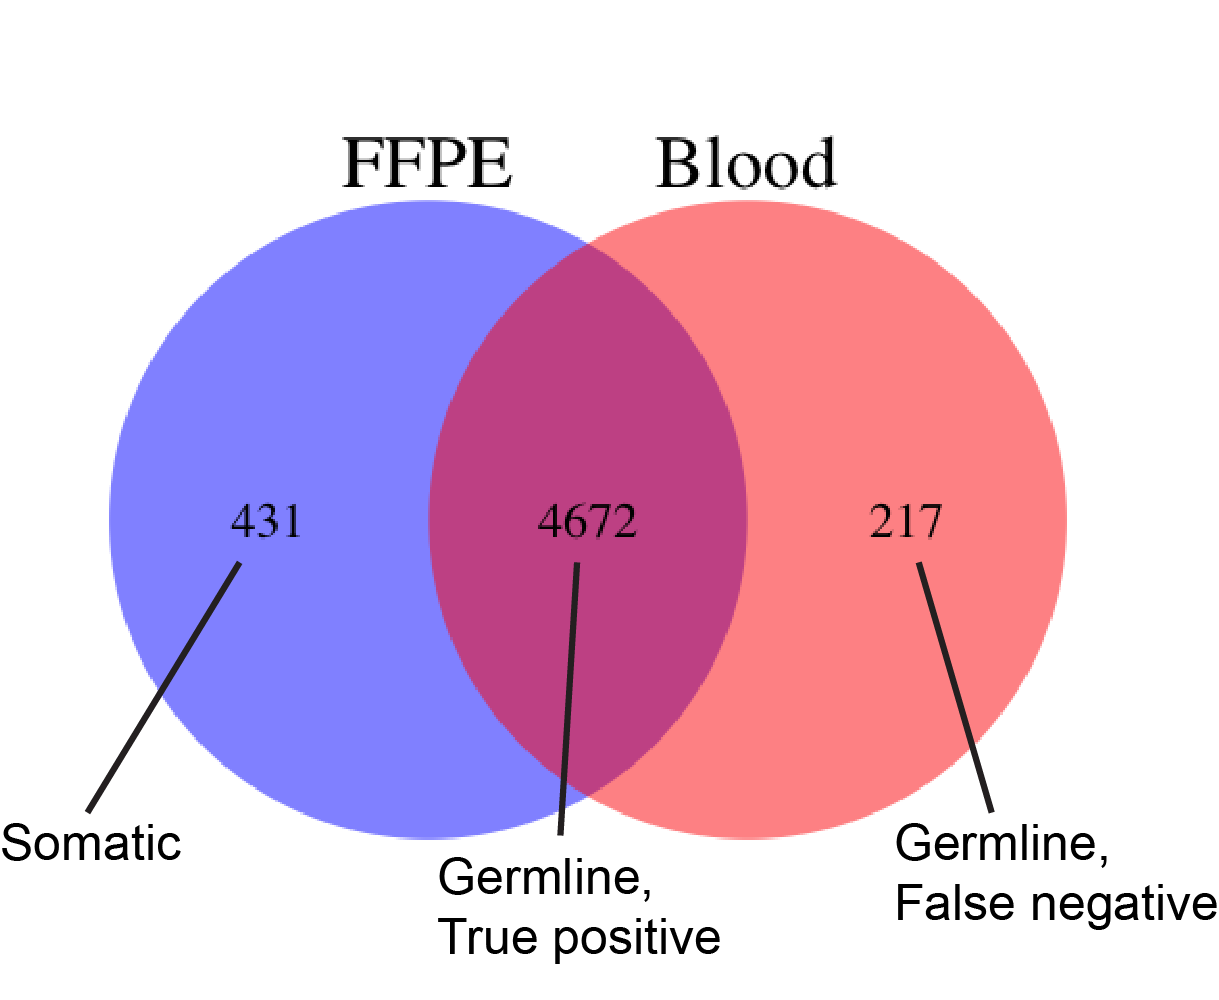
\includegraphics[scale=0.6]{variant_conc_venn.png}
	\caption{Add caption.}
	\label{fig:variant_conc_venn}
\end{figure}

\begin{figure}[H]
\centering
	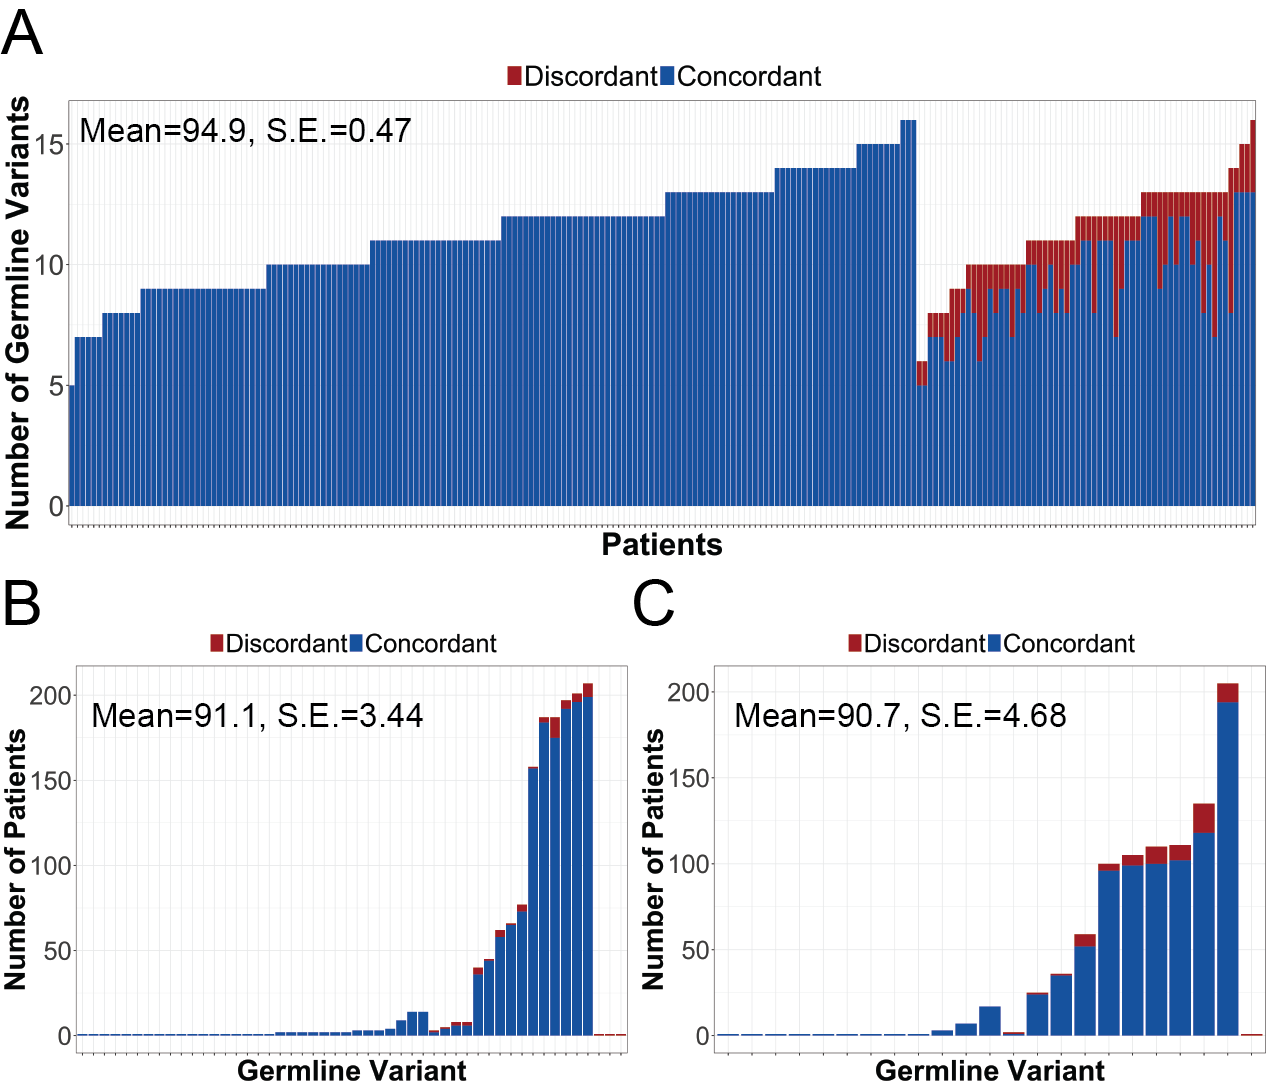
\includegraphics[scale=0.79]{true_positive_rate_variants.png}
	\caption{Add caption.}
	\label{fig:true_positive_rate_variants}
\end{figure}


%%%%%%%%%%%%%%%%%%%%%%%%%%%%%%%%%%%%%%%%%%%%%%%%%%%%%%%%%%%%%%%%%%%%%%
\section{Bioinformatics approaches for discriminating between germline and somatic variants in FFPE tumours}
\label{sec:BioinformaticsapproachesfordiscriminatingbetweengermlineandsomaticstatusesofvariantsinFFPEtumours}


%%%%%%%%%%%%%%%%%%%%%%%%%%%%%%%%%%%%%%%%%%%%%%%%%%%%%%%%%%%%%%%%%%%%%%
\section{Reduced sensitivity is observed for detection of germline variants in FFPE specimens compared to blood}
\label{sec:ReducedsensitivityisobservedfordetectionofgermlinevariantsinFFPEspecimenscomparedtoblood}

\begin{figure}[H]
	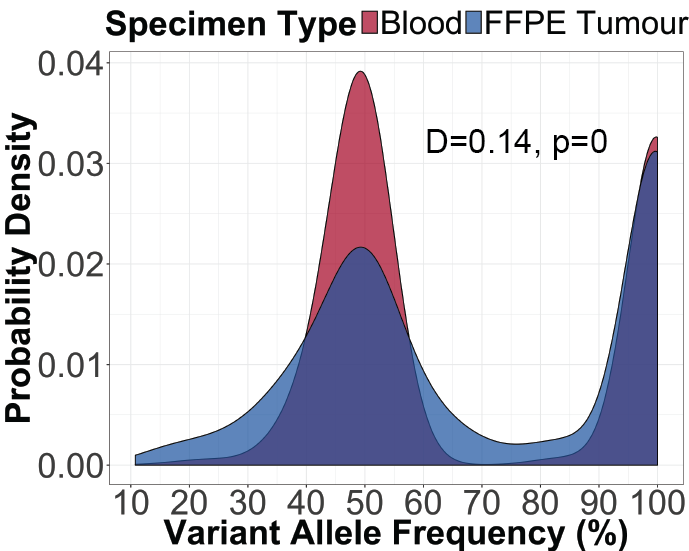
\includegraphics[scale=0.7]{germline_vaf_sens.png}
	\caption{Add caption.}
	\label{fig:germline_vaf_sens}
\end{figure}

\begin{table}[H]
\caption{Sensitivity of detecting germline variants in blood and FFPE specimens at various variant allele frequency thresholds.}
\label{sensitivity}
\centering
      \begin{tabular}{cllcclllccl}
        \hline
				\multicolumn{1}{l}{ }
				&
				\multicolumn{4}{l}{Blood}
				&&
				\multicolumn{4}{l}{FFPE Tumour}
        \\
				\cline{2-5}\cline{7-10}
        VAF (\%) & FN\mbox{*} & TP\mbox{**} & Sensitivity & 95\% CI && FN\mbox{*} & TP\mbox{**} & Sensitivity & 95\% CI
        \\
        \hline
        10 & 0 & 2461 & 1.0 & 1.0--1.0 && 0 & 2428 & 1.0 & 1.0--1.0
        \\
        15 & 2 & 2459 & 1.0 & 1.0-1.0 && 12 & 2416 & 1.0 & 0.99--1.0
        \\
        20 & 3 & 2458 & 1.0 & 1.0--1.0 && 48 & 2380 & 0.98 & 0.97--0.99
        \\
        25 & 15 & 2446 & 0.99 & 0.99--1.00 && 79 & 2349 & 0.97 & 0.96--0.97
        \\
        30 & 20 & 2441 & 0.99 & 0.99--1.00 && 121 & 2307 & 0.95 & 0.94--0.96
        \\
        35 & 33 & 2428 & 0.99 & 0.98--0.99 && 197 & 2231 & 0.92 & 0.91--0.93
        \\
        40 & 107 & 2354 & 0.96 & 0.95--0.96 && 328 & 2100 & 0.86 & 0.85--0.88
        \\
        45 & 234 & 2227 & 0.90 & 0.89--0.92 && 470 & 1958 & 0.81 & 0.79--0.82
        \\
				\hline
      \end{tabular} \\
\end{table}

\begin{figure}[H]
	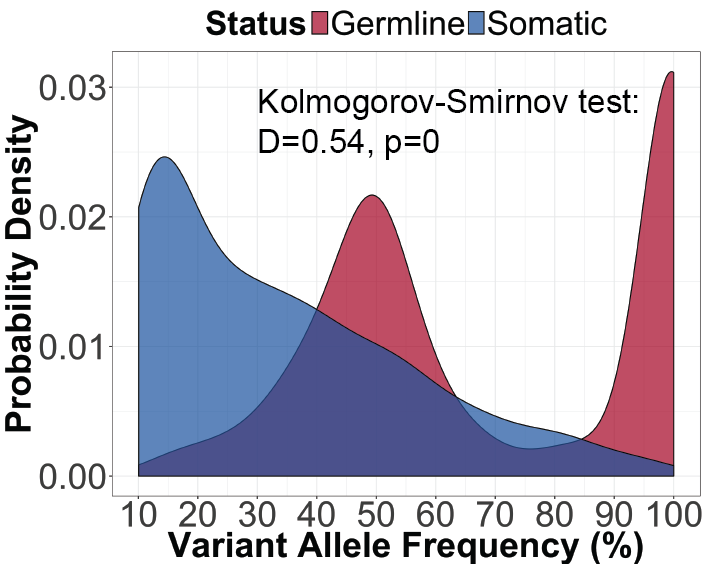
\includegraphics[scale=0.7]{germline_somatic_ppv.png}
	\caption{Add caption.}
	\label{fig:germline_somatic_ppv}
\end{figure}

\begin{table}[H]
\caption{Positive predictive value for referral of potential germline variants for downstream confirmatory testing.}
\label{ppv}
\centering
      \begin{tabular}{ccccccl}
        \hline
        VAF (\%) & False Positive & True Positive & Total Calls & Positive Predictive Value & 95\% CI
        \\
        \hline
        10 & 431 & 2428 & 2859 & 0.85 & 0.84--0.86
        \\
        15 & 319 & 2416 & 2735 & 0.88 & 0.87--0.90
        \\
        20 & 273 & 2380 & 2653 & 0.90 & 0.88--0.91
        \\
        25 & 245 & 2349 & 2594 & 0.91 & 0.89--0.92
        \\
        30 & 203 & 2307 & 2510 & 0.92 & 0.91--0.93
        \\
        35 & 178 & 2231 & 2409 & 0.93 & 0.91--0.94
        \\
        40 & 146 & 2100 & 2246 & 0.93 & 0.92--0.94
        \\
        45 & 118 & 1958 & 2076 & 0.94 & 0.93--0.95
        \\
				\hline
      \end{tabular} \\
\end{table}


%%%%%%%%%%%%%%%%%%%%%%%%%%%%%%%%%%%%%%%%%%%%%%%%%%%%%%%%%%%%%%%%%%%%%%
\section{Factors underlying reduced sensitivity of germline variant calling in FFPE specimens}
\label{sec:FactorsunderlyingreducedsensitivityofgermlinevariantcallinginFFPEspecimens}

%%%%%%%%%%%%%%%%%%%%%%%%%%%%%%%%%%%%%%%%%%%%%%%%%%%%%%%%%%%%%%%%%%%%%
\section{Discussion}
\label{sec:Discussion}
%%%%%%%%%%%%%%%%%%%%%%%%%%%%%%%%%%%%%%%%%%%%%%%%%%%%%%%%%%%%%%%%%%%%%

\endinput
\pagebreak
\begin{table}[H]
\caption{Frequency of germline and somatic variants detected in the tumours of 213 patients in the TOP cohort.}\label{freqvariants}
\centering
\begin{tabular}{lcclcl}
        \hline
        Gene & Germline & Pathogenic Germline && Somatic \\
				 & (N Patients) & (N Patients) && (N Patients) \\
				\hline
				\\
				\multicolumn{1}{l}{\textit{Cancer predisposing}}
				&
				\multicolumn{2}{l}{ }
				&&
				\multicolumn{1}{l}{} \\
				\hline
				AKT1 & 0 & 0 && 2 (2) \\
				\arrayrulecolor{evagrey}\hline
				ALK & 1 (1) & 1 (1) && 2 (1) \\
				\hline
				BRAF & 0 & 0 && 18 (17) \\
				\hline
				EGFR & 170 (164) & 5 (5) && 31 (24) \\
				\hline
				HRAS & 0 & 0 && 1 (1) \\
				\hline
				MAP2K1 & 0 & 0 && 2 (2) \\
				\hline
				MAPK1 & 17 (17) & 3 (3) && 3 (2) \\
				\hline
				MTOR & 763 (213) & 6 (6) && 71 (30) \\
				\hline
				NRAS & 0 & 0 && 8 (8) \\
				\hline
				PDGFRA & 242 (185) & 0 && 8 (4) \\
				\hline
				PIK3CA & 0 & 0 && 15 (4) \\
				\hline
				PTEN & 0 & 0 && 1 (1) \\
				\hline
				STAT1 & 54 (51) & 1 (1) && 7 (6) \\
				\hline
				STAT3 & 10 (10) & 4 (4) && 16 (11) \\
				\hline
				TP53 & 189 (184) & 2 (2) && 131 (109) \\
				\arrayrulecolor{black}\hline
				\\
				\multicolumn{1}{l}{\textit{Pharmacogenomics}}
				&
				\multicolumn{2}{l}{ }
				&&
				\multicolumn{1}{l}{} \\
				\arrayrulecolor{black}\hline
				DPYD & 271 (212) & 1 (1) && 1 (1) \\
				\arrayrulecolor{evagrey}\hline
				GSTP1 & 106 (106) & 0 && 0 \\
				\hline
				MTHFR & 209 (177) & 0 && 0 \\
				\hline
				TYMP & 81 (76) & 2 (2) && 18 (13)\\
				\hline
				TYMS & 131 (131) & 0 && 0 \\
				\hline
				UGT1A1 & 96 (96) & 0 && 1 (1) \\
				\arrayrulecolor{black}\hline \\
				Total & 2396 (213*) & 25 (23*) && 431 (180*) \\
				\arrayrulecolor{black}\hline
      \end{tabular}
\end{table}
